\documentclass[12pt]{report}
\usepackage{setspace}
\usepackage[utf8]{inputenc}
\usepackage[titletoc]{appendix}
\usepackage{graphicx}
\usepackage{listings}
\graphicspath{ {images/} }
\setlength{\parindent}{0pt}
\setlength{\parskip}{1em}
\usepackage{float}
\usepackage{multirow}
\usepackage{booktabs}

% hyperlinks
\usepackage{hyperref} 
\hypersetup{ colorlinks, citecolor=red, filecolor=black, linkcolor=black, urlcolor=blue } 

% blank page
\usepackage{afterpage}
\newcommand\blankpage{%
    \null
    \thispagestyle{empty}%
    \addtocounter{page}{-1}%
    \newpage}

\usepackage{pgf}
\usepackage{pgfpages}

% Border
\pgfpagesdeclarelayout{boxed}
{
  \edef\pgfpageoptionborder{0pt}
}
{
  \pgfpagesphysicalpageoptions
  {%
    logical pages=1,%
  }
  \pgfpageslogicalpageoptions{1}
  {
    border code=\pgfsetlinewidth{0.5pt}\pgfstroke,%
    border shrink=\pgfpageoptionborder,%
    resized width=.95\pgfphysicalwidth,%
    resized height=.95\pgfphysicalheight,%
    center=\pgfpoint{.5\pgfphysicalwidth}{.5\pgfphysicalheight}%
  }%
}
\pgfpagesuselayout{boxed}

% page layout including header and footer
\usepackage{xcolor}
\usepackage[a4paper,top=2cm, bottom=3.5cm, left=2.54cm, right=2.54cm]{geometry}
\definecolor{myred}{HTML}{581000}
\usepackage{fancyhdr}
\pagestyle{fancy}
% \fancyhead{}
% \fancyhead[L]{\slshape\nouppercase{\leftmark}}
% \fancyhead[R]{\slshape\nouppercase{\rightmark}}
\fancyfoot{}
\fancyfoot[R]{\thepage}
\fancyfoot[L]{\textbf{Department of Electronics Engineering 2017-21 Batch}}
% \renewcommand{\headrulewidth}{0.5pt}
\renewcommand{\footrulewidth}{3pt}
\renewcommand{\footrule}{\hbox to\headwidth{\color{myred}\leaders\hrule height \footrulewidth\hfill}}
\usepackage{caption}
\usepackage{subcaption}
\setcounter{page}{1}
\setcounter{chapter}{0}
\fancypagestyle{plain}{%
\fancyhf{}% clear all header and footer fields
\fancyfoot{}
\fancyfoot[R]{\thepage}
\fancyfoot[L]{\textbf{Department of Electronics Engineering 2017-21 Batch}}
% \renewcommand{\headrulewidth}{0.5pt}
\renewcommand{\footrulewidth}{3pt}
\renewcommand{\footrule}{\hbox to\headwidth{\color{myred}\leaders\hrule height \footrulewidth\hfill}}
}

% table format
\usepackage{array}
\newcolumntype{Y}{>{\centering\arraybackslash}m{4.4cm}}
\newcolumntype{X}{>{\centering\arraybackslash}m{7cm}}
\newcolumntype{P}{>{\centering\arraybackslash}m{2.5cm}}
\newcolumntype{L}{>{\raggedright\arraybackslash}m{8cm}}
\newcolumntype{M}{>{\raggedright\arraybackslash}m{3.7cm}}
\newcolumntype{Z}{>{\justify}m{15cm}}

% references
\usepackage{biblatex}
\addbibresource{references.bib}

\title{
{Design and Implementation of Vehicle Control Unit in Formula Student Electric race-car}}
\author{Arpan Biswas, 1712006 \\ Vraj Brahmbhatt, 1712007}
\date{2021}

\usepackage{nomencl}
\makenomenclature

\begin{document}

% page no. roman
\renewcommand{\thepage}{\roman{page}}



\begin{titlepage}
    \begin{center}
        \vspace*{0.1cm}
          
        \LARGE
        \textbf{University of Mumbai}
        \vspace{0.5cm}
        
        \LARGE
        \textbf{Design and Implementation of Vehicle Control Unit in Formula Student Electric race-car}
         
        \par 
        \large
        Submitted in partial fulfillment of requirements\\
        for the degree of\\
        \Large
        \par
        \textbf{Bachelors in Technology}
        
        \large
        \par
        by
        
        \Large
        \par
        \textbf{Arpan Biswas\\ Roll No: 1712006,\\ \vspace{0.5cm} Vraj Brahmbhatt\\ Roll No: 1712007}\\
        
        \large
        \vspace{0.5cm}
        Guide:\\
        \Large
        \textbf{Prof. Anil S. Thosar}
            
        \vfill
            
        \vspace{0.5cm}
            
        
\includegraphics[width=0.2\textwidth]{KJSCE logo.jpg}\\
        \vspace{0.5cm}   
        \large
        \textbf{Department of Electronics Engineering}\\
        \textbf{K.J. Somaiya College of Engineering, Mumbai-77}\\
        \normalsize
        \textbf{(Autonomous College Affiliated to University of Mumbai)}\\
        \vspace{0.5cm}
        \large
        \textbf{Batch 2017-2021}\\
        \vspace{0.8cm}

    \end{center}
\end{titlepage}

\setstretch{1.5}

% \begin{certi}

    \begin{center}
    
        \vspace*{0.1cm}
        \large
        \textbf{K.J. Somaiya College of Engineering, Mumbai-77}\\
        \normalsize
        (Autonomous College Affiliated to University of Mumbai)\\
        
        \vspace{0.8cm}
        
        \large
        \textbf{Certificate}\\
        \vspace{0.5cm}
        
    \end{center}
% \end{certi}
\noindent
{\large This is to certify that the dissertation report entitled \textbf{*insert project name*} submitted by Author Name and Co-author Name at the end of semester VIII of LY B. Tech is a bona fide record for partial fulfillment of requirements for the degree of Bachelors of Technology in Electronics Engineering of University of Mumbai.}
\vspace{2cm}

\begin{table}[h]
\centering
\begin{tabular}{Y Y Y}
\hrulefill & & \hrulefill \\
\large Guide & & \large Head of Department \\
\end{tabular}
\end{table}

\vspace{2cm}

\begin{table}[h]
\centering
\begin{tabular}{Y Y Y}
\hrulefill & & \\
\large Principal & & \\
\end{tabular}
\end{table}

\vspace{1cm}
\noindent
{\large Date:}\\
{\large Place: Mumbai-77}



\newpage
    \begin{center}
    
        \vspace*{0.1cm}
        \large
        \textbf{K.J. Somaiya College of Engineering, Mumbai-77}\\
        \normalsize
        (Autonomous College Affiliated to University of Mumbai)\\
        
        \vspace{0.8cm}
        
        \large
        \textbf{Certificate of Approval of Examiners}\\
        \vspace{0.5cm}
        
    \end{center}

\noindent
{\large We certify that this dissertation report entitled \textbf{*insert project name*} is bona fide record of project work done by Author Name and Co-author name. This project is approved for the award of Bachelors in Technology Degree in Electronics Engineering of University of Mumbai.} 
\vspace{2cm}

\begin{table}[h]
\centering
\begin{tabular}{Y}
\hrulefill\\
\large Internal Examiner\\
\end{tabular}
\end{table}

\vspace{2cm}

\begin{table}[h]
\centering
\begin{tabular}{Y}
\hrulefill\\
\large External Examiner
\end{tabular}
\end{table}

\vspace{1cm}
\noindent
{\large Date:}\\
{\large Place: Mumbai-77}

% \begin{certi}
\newpage
    \begin{center}
    
        \vspace*{-1cm}
        \large
        \textbf{K.J. Somaiya College of Engineering, Mumbai-77}\\
        \normalsize
        (Autonomous College Affiliated to University of Mumbai)\\
        
        \vspace{0.8cm}
        
        \large
        \textbf{DECLARATION}\\
        \vspace{0.5cm}
        
    \end{center}
% \end{certi}
\noindent
{We declare that this written thesis submission represents the work done based on our and / or others’ ideas with adequately cited and referenced the original source. We also declare that we have adhered to all principles of intellectual property, academic honesty and integrity as we have not misinterpreted or fabricated or falsified any idea/data/fact/source/original work/ matter in my submission. \par

We understand that any violation of the above will be cause for disciplinary action by the college and may evoke the penal action from the sources which have not been properly cited or from whom proper permission is not sought.}

\begin{table}[h]
\centering
\begin{tabular}{| X | X |}
\hline
 & \\
 & \\
\hrulefill & \hrulefill \\
\textbf{Signature of the Student} & \textbf{Signature of the Student} \\
\vspace{4cm} & \vspace{4cm} \\
 & \\
\textbf{1712006} & \textbf{1712007} \\
\hrulefill & \hrulefill \\
\textbf{Roll No.} & \textbf{Roll No.} \\
\hline
 & \\
 & \\
\hrulefill & \\
\textbf{Signature of the Student} & \\
\vspace{4cm} & \\
 & \\
\textbf{1712006} &  \\
\hrulefill &  \\
\textbf{Roll No.} & \\
\hline
\end{tabular}
\end{table}


\noindent
{\large Date:}\\
{\large Place: Mumbai-77}


\addcontentsline{toc}{chapter}{Abstract}
\newpage
    \begin{center}
    
        \vspace*{0.05cm}
        \Large
        \textbf{Abstract}\\
        \vspace{0.5cm}
        
    \end{center}

Some text ...


\setlength{\parskip}{0pt}
\tableofcontents
\addcontentsline{toc}{chapter}{List of Figures}
\listoffigures
\addcontentsline{toc}{chapter}{List of Tables}
\listoftables


\addcontentsline{toc}{chapter}{Nomenclature}
% \newpage
%     \begin{center}
    
%         \vspace*{0.1cm}
%         \Large
%         {Nomenclature}\\
%         \vspace{0.5cm}
        
%     \end{center}

% \begin{tabular}{ l l }
%  BMS & Battery Management System \\ 
%  isoSPI & Isolated SPI communication \\
%  OCV & Open-Circuit Voltage\\
%  PEC & Packet Error Code\\
%  HV	& High Voltage\\
%  LV	& Low Voltage\\
%  SAE & Society of Automotive Engineers\\
%  AUTOSAR & AUTomotive Open System ARchitecture\\
%  VCU & Vehicle Control Unit\\
%  ECU & Electronic Control Unit\\
%  EMI & Electromagnetic Interference\\
%  RWD & Rear Wheel Drive\\
%  LCS & Launch Control System\\
%  TCS & Traction Control System\\
%  PMSM & Permanent-Magnet Synchronous Motor\\
%  CAN & Controller Area Network\\
%  SPI & Serial Peripheral interface\\
%  UART & Universal Asynchronous Receiver/Transmitter\\
%  GPS & Global Positioning System\\
%  IMU & Inertial Measurement Unit\\
%  EKF & Extended Kalman Filter\\
%  PCB & Printed Circuit Board\\
%  DOF & Degree of Freedom\\
%  PID & Partial Integral Derivative \\
%  DAQ & Data Acquisition \\
%  LCD & Liquid Crystal Display \\
%  GUI & Graphical User Interface \\
% \end{tabular}

\mbox{}

\nomenclature{XYZ}{xxx yyy zzz}


\printnomenclature
% \afterpage{\blankpage}



%%%%%%%%%%%%
% Chapters

% page number numeric
\clearpage
\setcounter{page}{1}
\setcounter{chapter}{0}
% main page numbers:  1, 2, 3, ...
\renewcommand{\thepage}{\arabic{page}}	

\setlength{\parskip}{1em}

\chapter{Introduction}\label{cha:introduction}
For reference see figure \ref{fig:artemis}, equation \ref{eq:pid}, and table \ref{tab:myrio}. For citations use \cite{FSG}.

\begin{figure}[hbt!]
    \centering
    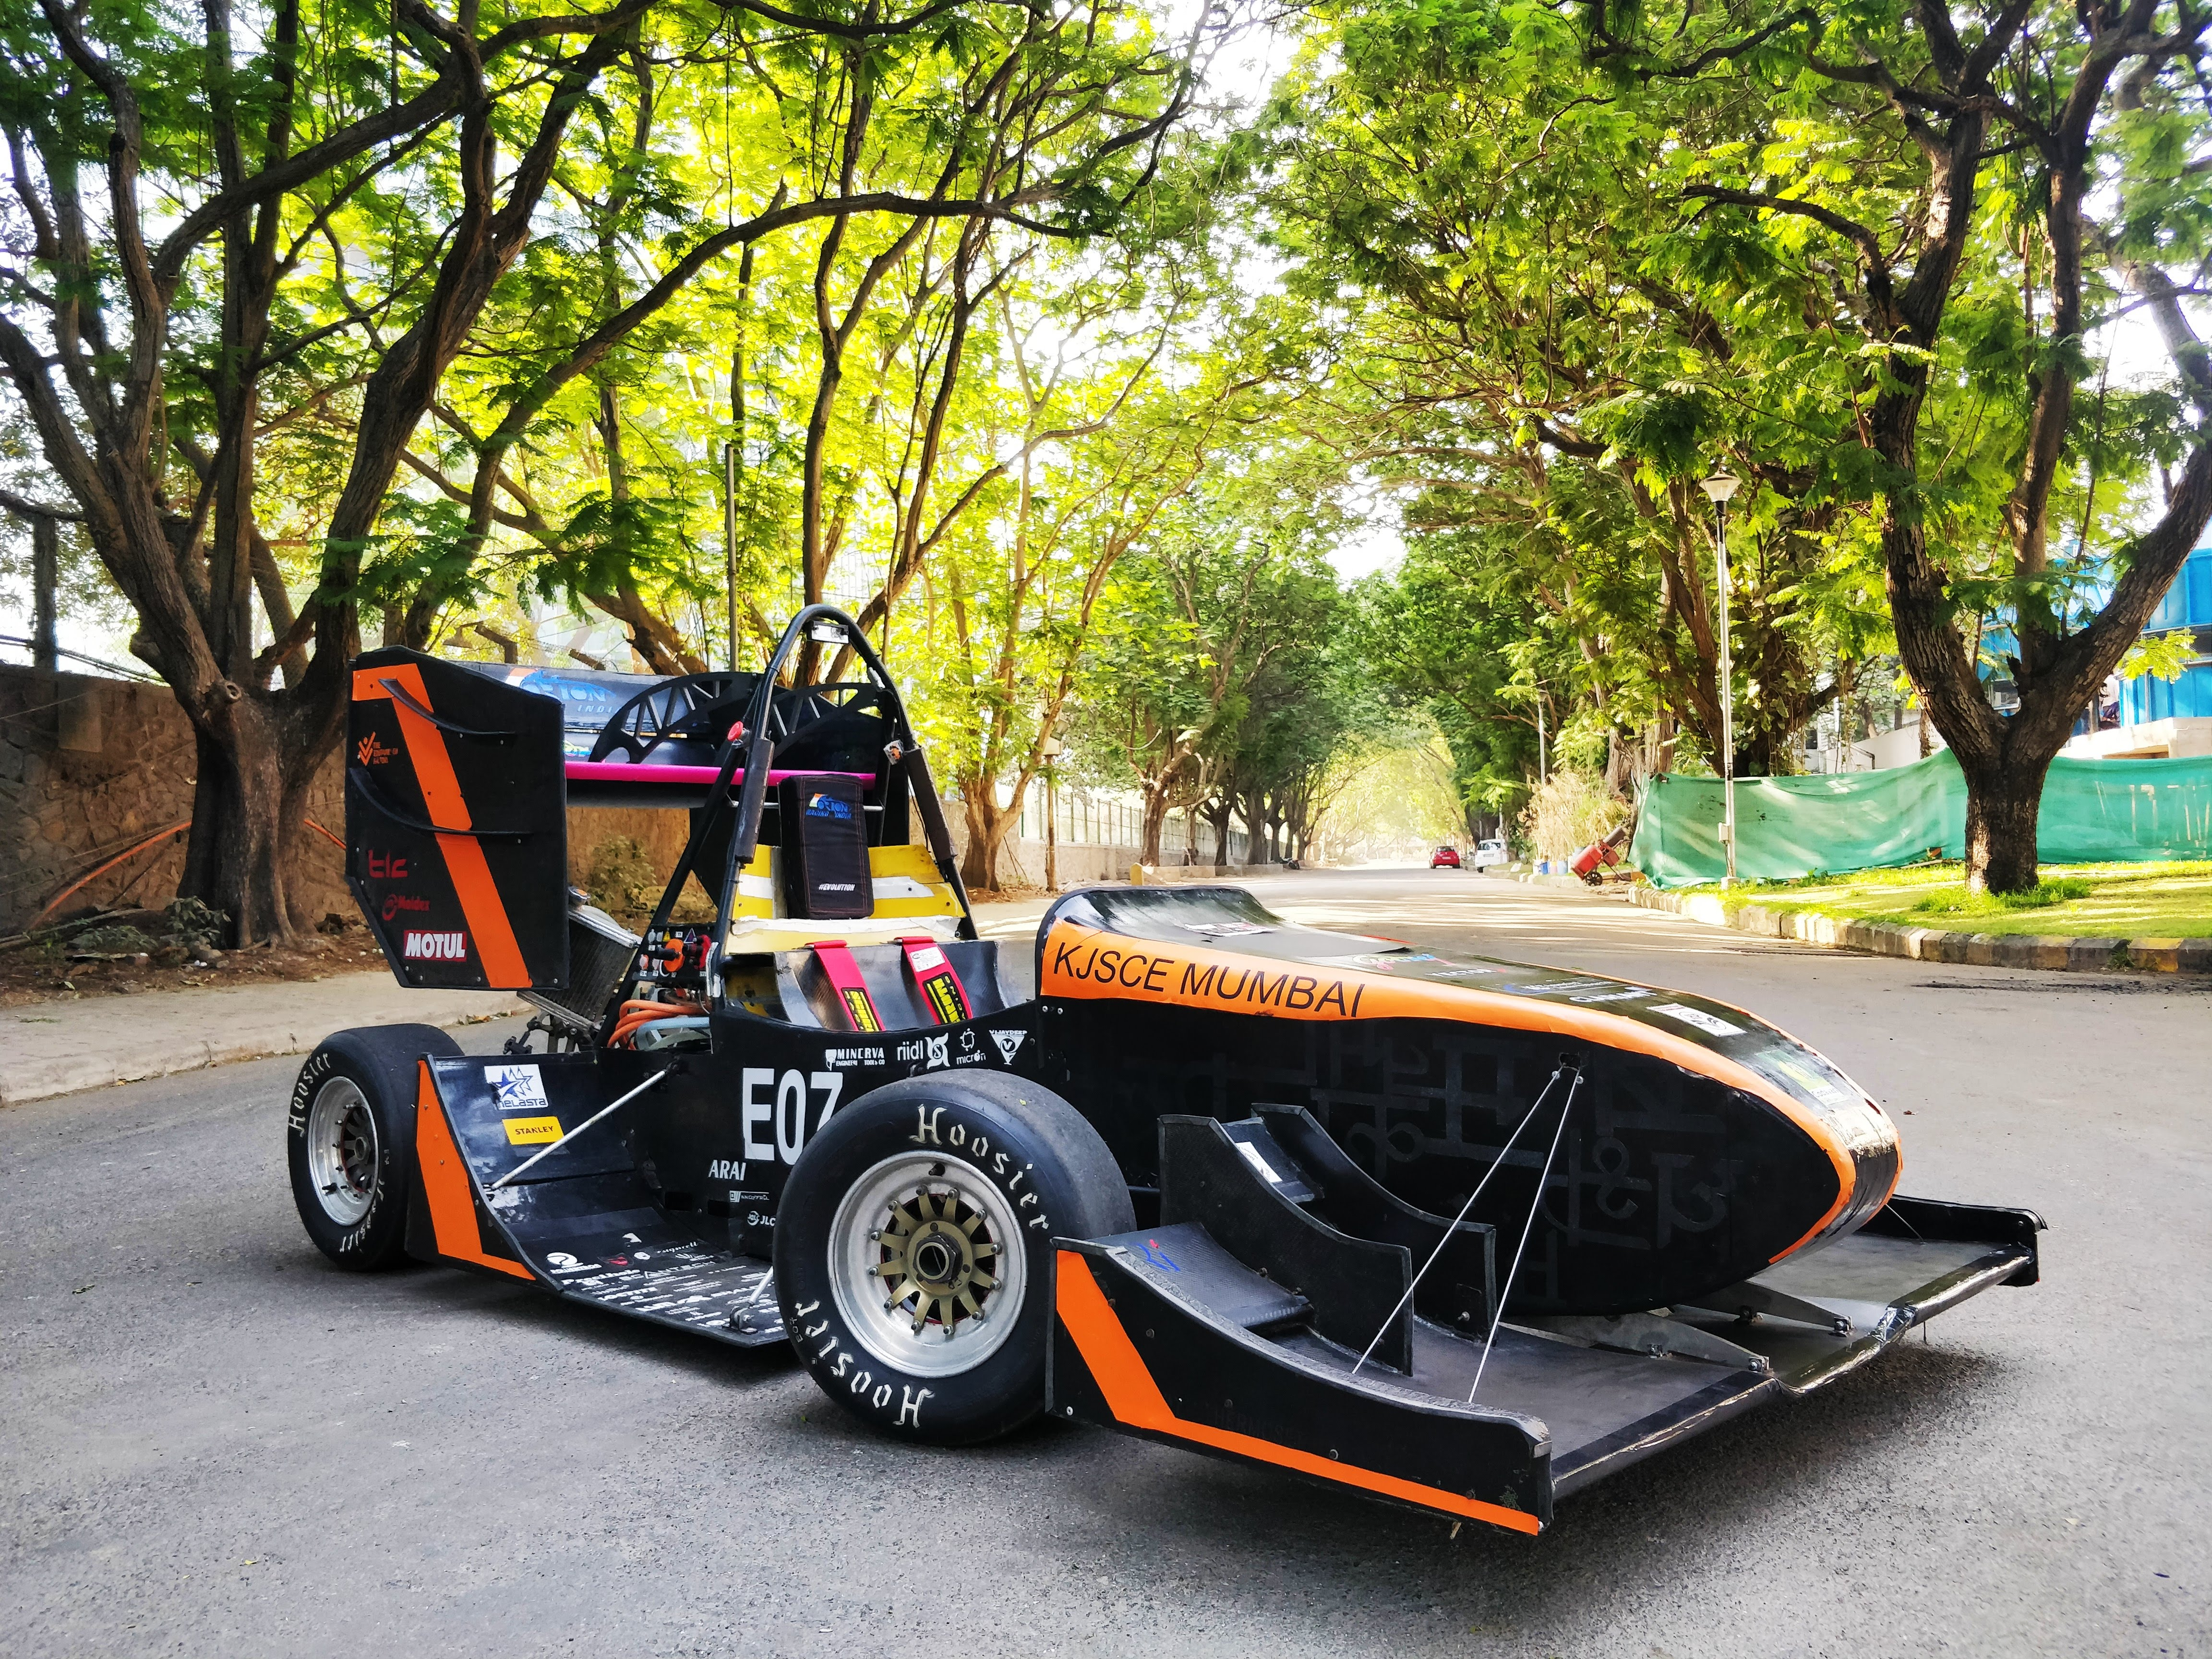
\includegraphics[width=0.8\textwidth]{images/Artemis.jpg}
    \caption{Artemis (ORI19e)}\label{fig:artemis}
\end{figure}

\[u(t) = K_p \ e(t) + K_i\ \int_{t_0}^{t} e(t') \ dt' + K_d \ \frac{de(t)}{dt}\] \label{eq:pid}

\begin{table}[hbt!]
\begin{center}
\scalebox{1}{%
\begin{tabular}{|M|L|}
 \hline
 \textbf{Components} & \textbf{Figures} \\
 \hline
 Processor & Xilinx FPGA and dual-core ARM Cortex-A9 processor \\ 
 \hline
 Max. Processor Operating Frequency & 667 MHz \\
 \hline
 Operating voltage & 6V - 16V \\
 \hline
 Program memory & 256 MB, DDR3 \\
 \hline
 Data memory & 512 MB, 533 MHz, 16 bits \\
 \hline
 Digital GPIOs & 40 \\
 \hline
 Analog pins & 10 (Input, 12-bit resolution), 6 (Output, 12-bit resolution) \\
 \hline
 Preferred programming language & LabVIEW \\
 \hline
 Max power consumption & 14 W \\
 \hline
 Wireless & IEEE 802.11/b/g/n ISM 2.4 GHz \\
 \hline
 USB & 2.0 Hi-Speed  \\
 \hline
 Inbuilt sensor & 3 axis accelerometer\\
 \hline
\end{tabular}}
\caption{\label{tab:myrio}NI myRIO important figures}
\end{center}
\end{table}


\chapter{Literature review\label{cha:litreivew}}\label{chap:lit}
\vspace{-0.8cm}
\noindent\fbox{%
    \parbox{\textwidth}{%
        This chapter presents ...
        \\
        \\
    }%
}

\section{Section 1}
Some text ...

\subsection{Sub-section 1}
Some text ...

\subsection{Sub-section 2}
Some text ...

\chapter{Project design\label{cha:design}}
\vspace{-0.8cm}
\noindent\fbox{%
    \parbox{\textwidth}{%
        This chapter presents ...
        \\
        \\
    }%
}

\section{Section 1}
Some text ...

\subsection{Sub-section 1}
Some text ...

\subsection{Sub-section 2}
Some text ...

\chapter{Implementation and experimentation\label{cha:implementation}}
\vspace{-0.8cm}
\noindent\fbox{%
    \parbox{\textwidth}{%
        This chapter presents ...
        \\
        \\
    }%
}

\section{Section 1}
Some text ...

\subsection{Sub-section 1}
Some text ...

\subsection{Sub-section 2}
Some text ...

\chapter{Results}
\vspace{-0.8cm}
\noindent\fbox{%
    \parbox{\textwidth}{%
        This chapter presents ...
        \\
        \\
    }%
}

\section{Section 1}
Some text ...

\subsection{Sub-section 1}
Some text ...

\subsection{Sub-section 2}
Some text ...

\chapter{Conclusions and scope for further work}
\input{chapters/conclusion}

\addcontentsline{toc}{chapter}{Bibliography}
\printbibliography

\appendix
% \chapter{Appendix}
\begin{appendices}
  \chapter{Appendix}
  
  
\end{appendices}

\newpage
\thispagestyle{plain}
    \begin{center}
    
        \vspace*{0.1cm}
        \Large
        \textbf{Acknowledgements}\\
        \vspace{0.5cm}
        
    \end{center}

Some text ...
\addcontentsline{toc}{chapter}{Acknowledgements}

\end{document}
